% Standalone evaluation report (self-contained).
% Build from the evaluation/ directory:
%   pdflatex evaluation_standalone.tex && pdflatex evaluation_standalone.tex
% Regenerate the \input-ed tables/figures first:
%   python ../evaluation/run_evaluation.py --full
%   python ../figures/make_servicedesk_petrinets.py   (Petri-net case-study figure)
%
% Compact house-style version: 1 body figure + 4 tables, no RQ tags, limitations
% folded into the close.  A short appendix keeps the 10-panel noise figure and the
% case-weighted quality table.  Result numbers are written into the prose.

\documentclass[10pt]{article}
\usepackage[a4paper,margin=2cm]{geometry}
\usepackage{amsmath,amssymb}
\usepackage{graphicx}
\usepackage{booktabs}
\usepackage{caption}
\usepackage{subcaption}
\usepackage{enumitem}
\usepackage{multicol}
\usepackage[hidelinks]{hyperref}
\graphicspath{{figures/}}
\captionsetup{font=small,labelfont=bf,skip=4pt}
\setlist{nosep,leftmargin=1.4em}
\setlength{\parskip}{0.35em}
\setlength{\parindent}{0pt}
\pagestyle{plain}

\title{Discovering Hidden Process Views from Translucent Event Logs\\[2pt]
\large Evaluation}
\author{Harry H.\ Beyel \and Wil M.\ P.\ van der Aalst}
\date{}

\begin{document}
\maketitle
\vspace{-2.2em}

\begin{abstract}
\noindent We evaluate the relationship-induced abstraction $\kappa$ in three steps: whether it \emph{recovers} the hidden view-defining context, whether its per-view models are \emph{better} than global discovery, trace clustering, and variant discovery, and how it behaves in a realistic \emph{case study} where the recorded enabled activities carry noise.
Across nine synthetic logs $\kappa$ recovers the hidden context exactly (ARI $1.00$), parameter-free, and its per-view models are the most faithful to the enabled behaviour among the compact approaches.
Its one weakness is made explicit: $\kappa$ reads structure only from the enabled sets, so corrupting them degrades it sharply while control-flow clustering is unaffected but never competitive.
\end{abstract}

\section{Evaluation}
\label{sec:evaluation}
We evaluate the relationship-induced abstraction $\kappa$ (Section~4) in three steps that mirror the three claims of the introduction: whether $\kappa$ \emph{recovers} the hidden view-defining context, whether its per-view models are \emph{better} than global discovery, trace clustering, and variant discovery, and how it behaves in a realistic \emph{case study} where the recorded enabled activities carry noise.
All experiments use synthetic translucent event logs, so the hidden context is known and recovery can be measured exactly; reported numbers are means over three random seeds.
Our implementation and the evaluation pipeline are publicly available;\footnote{\url{https://github.com/hherbertb/translucent-process-views}} everything is implemented in Python with PM4Py~\cite{vanderaalst2016}.

\subsection{Experimental setup}
\label{sec:setup}

\paragraph{Synthetic logs.}
Each generator fixes one control-flow skeleton over a small activity alphabet --- a spine of activities with a few \emph{flexible blocks} (a set of choices, an optional step) --- and a \emph{hidden label} that sets how each block behaves: a block of choices is resolved concurrently, in a fixed order, or is pinned to one branch; and an optional step is present or absent.
To generate a case we draw one hidden label and emit a random trace consistent with it, recording at every event both the executed activity and the set of activities that were selectable (its enabled set); the label is then removed, so it survives only in the pattern of enabled sets, which is what $\kappa$ reads.
Each generator is tuned so that all variants of one hidden label collapse onto a \emph{single} $\kappa$ identifier while different labels get different identifiers.
Table~\ref{tab:logs} lists the nine logs; each isolates one phenomenon, stated in its group header.
The \emph{$k$-view} family is the controlled sweep --- one base process in two to five configurations --- and varies the ground-truth $k$; each of the other five logs adds one axis $k$-view does not exercise.
\emph{Running example} is the paper's running example $L_{\mathrm{run}}$ at scale: eight activities --- open ($o$), a check ($b$ or $c$), an assessment ($d$ or $e$), submit ($f$), approve ($g$) or reject ($h$) --- whose hidden label offers the two choices concurrently, sequentially, or pinned to one branch.
Scaling its six traces to $1500$ cases leaves the three abstraction identifiers unchanged, so $\kappa$ must return exactly $\mathit{seq}(o,\mathit{and}(\mathit{xor}(b,c),\mathit{xor}(d,e)),f,\mathit{xor}(g,h))$, $\mathit{seq}(o,\mathit{xor}(b,c),\mathit{xor}(d,e),f,\mathit{xor}(g,h))$, and $\mathit{seq}(o,b,d,f,\mathit{xor}(g,h))$.
\emph{Parallel choices} keeps the executed sequences identical across labels, so only the enabled sets can separate them and control-flow clustering cannot succeed even in principle; \emph{enterprise} scales the setting to ${\sim}20$ activities and five roles; \emph{role split} is the minimal clean case (six classical variants) and the only log where a hidden label skips activities entirely; and \emph{rework loop} has no hidden context at all --- the honest failure, where $\kappa$ over-segments an unbounded loop.
The column \textbf{hidden $k$} is the number of distinct hidden labels the generator used (``--'' when there is no hidden context) and \textbf{$\kappa$ views} is the number of equivalence classes $\kappa$ induces; the two coincide on every log with a hidden context and diverge only for \emph{rework loop}, which has none and where $\kappa$ unrolls the loop into four length-indexed views.

\begin{table}[t]
  \centering
  \caption{The nine synthetic logs and the phenomenon each isolates (group headers).
  Right of the rule is a result: $\kappa$ produces exactly hidden-$k$ views on every log except the rework loop.}
  \label{tab:logs}
  \small\setlength{\tabcolsep}{4pt}
  \begin{tabular}{lrrrrrr|r}
\toprule
log & cases & acts & avg\ len & class.\ var. & transl.\ var. & hidden $k$ & $\kappa$ views \\
\midrule
running example & 1500 & 8 & 5.0 & 16 & 26 & 3 & 3 \\
$k$-view ($k{=}2$) & 800 & 8 & 5.0 & 48 & 56 & 2 & 2 \\
$k$-view ($k{=}3$) & 1200 & 8 & 5.0 & 48 & 57 & 3 & 3 \\
$k$-view ($k{=}4$) & 1600 & 8 & 4.2 & 49 & 58 & 4 & 4 \\
$k$-view ($k{=}5$) & 1800 & 9 & 4.6 & 57 & 66 & 5 & 5 \\
parallel choices & 2000 & 13 & 8.0 & 390 & 535 & 5 & 5 \\
enterprise & 3000 & 21 & 11.8 & 2304 & 2503 & 5 & 5 \\
role split & 1040 & 7 & 5.6 & 6 & 8 & 3 & 3 \\
rework loop & 600 & 5 & 5.0 & 4 & 4 & -- & 4 \\
\bottomrule
\end{tabular}

\end{table}

\paragraph{Baselines.}
We compare $\kappa$ with eight alternatives.
\emph{Global} discovery mines one model from the whole log with the translucent Inductive Miner (IMtf)~\cite{beyel2024tar}.
\emph{Variant discovery} groups traces by their executed projection~\cite{greco2006,garciabanuelos2014}, and \emph{translucent-variant grouping} refines this to one group per distinct translucent trace.
\emph{Control-flow trace clustering} (CF-TC)~\cite{song2008} clusters activity-count and directly-follows features with $k$-means and Ward linkage; \emph{context-aware} clustering (CTX-TC)~\cite{bose2009} adds enabled-activity features and \emph{enabled-only} clustering (EN-TC) uses those alone.
\emph{Representation-learning} clustering (D2V-TC)~\cite{dekoninck2018} embeds each trace with Doc2Vec~\cite{lemikolov2014}, and \emph{attribute} clustering (ATTR-TC) clusters on recorded case attributes: four \emph{clean} ones that carry information about the hidden label --- \texttt{role} has normalised mutual information $1.00$ with it, \texttt{department} $0.55$, \texttt{location} $0.47$, \texttt{seniority} $0.19$ --- and six \emph{noisy} ones independent of it (all $\le 0.003$).
The tables list the $k$-means and Ward variants of CF-TC and the clean / noisy / all variants of ATTR-TC separately, each run with $k$ set to the ground-truth number of views (GT) and with $k$ chosen by the silhouette~\cite{rousseeuw1987} (auto).

\paragraph{Metrics.}
Each partition is compared with the hidden-label partition by the adjusted Rand index (ARI), normalised mutual information (NMI), and purity; all three lie in $[0,1]$ and are $1$ for a perfect match.
\emph{Enabled-signature incoherence} is the mean number of distinct per-position enabled-set sequences per (group, classical variant) pair; it is $1$ iff no group mixes availability contexts.
For \emph{model quality} we discover one model per group with IMtf and score it on its own sub-log: fitness (alignments~\cite{adriansyah2014}), precision (alignment-based~\cite{carmona2018}), generalisation, simplicity (net size), and the enabled-set-aware translucent fitness / precision~\cite{beyel2024tp,beyel2025ta}; F1 is the harmonic mean of fitness and precision.
Because several models are discovered per log, the per-log score is the case-frequency-weighted mean over the groups and the reported value is the unweighted mean over the nine logs (the case-weighted variant is in Table~\ref{tab:quality-cw}).
The model-quality experiment uses one seed; the partition metrics average three.

\subsection{Recovering hidden context}
\label{sec:recovery}
Table~\ref{tab:recovery} reports, for every grouping and given the ground-truth $k$, whether its groups are the right ones.
Global discovery yields one group and recovers nothing; variant and translucent-variant grouping produce $325$ and $368$ groups for a hidden $k$ of at most five, and their groups still mix $1.24$ enabled-activity signatures per (group, variant) against $1.00$ for $\kappa$.
Given $k=\mathrm{GT}$, the control-flow, context-aware, enabled-only, and Doc2Vec baselines reach ARI $\le 0.53$ (and $\le 0.65$ with $k$ by silhouette), whereas $\kappa$ reaches ARI, NMI, and purity of $1.00$ with no cluster count, distance function, threshold, or clustering algorithm.
On the running example this is the paper's own answer: the three identifiers $\kappa$ induces are exactly the three listed above, one per hidden resolution, at ARI $1.00$ and $500$ cases each.
The only baseline that matches $\kappa$ is attribute clustering on the clean attributes (ARI $1.00$) --- and only because \texttt{role} was recorded and $k$ was supplied; on the noisy attributes it is at chance.

\begin{table}[t]
  \centering
  \caption{Recovering the hidden context: ARI / NMI / purity against the hidden label, and enabled-signature incoherence, for every grouping. \emph{GT} / \emph{auto} $=$ $k$ set to the true view count / chosen by silhouette. Mean over the nine logs and three seeds; the best value in each column is in \textbf{bold}.}
  \label{tab:recovery}
  \footnotesize\setlength{\tabcolsep}{5pt}
  \begin{tabular}{lrrrr}
\toprule
 & ARI & NMI & purity & enabl.\ sig. \\
\midrule
global & 0.000 & 0.000 & 0.303 & 1.236 \\
$\kappa$ (ours) & \textbf{1.000} & \textbf{1.000} & \textbf{1.000} & \textbf{1.000} \\
$\kappa$ + support (ours) & \textbf{1.000} & \textbf{1.000} & \textbf{1.000} & \textbf{1.000} \\
CF-TC $k$-means (GT) & 0.238 & 0.323 & 0.542 & 1.265 \\
CF-TC Ward (GT) & 0.331 & 0.446 & 0.636 & 1.265 \\
CTX-TC (GT) & 0.351 & 0.508 & 0.645 & 1.246 \\
EN-TC (GT) & 0.514 & 0.651 & 0.733 & 1.125 \\
D2V-TC (GT) & 0.470 & 0.556 & 0.689 & 1.061 \\
ATTR-TC clean (GT) & 0.799 & 0.867 & 0.851 & 1.021 \\
ATTR-TC noisy (GT) & 0.176 & 0.218 & 0.501 & 1.066 \\
ATTR-TC all (GT) & 0.636 & 0.733 & 0.774 & 1.038 \\
variant discovery & 0.251 & 0.400 & 0.852 & 1.236 \\
translucent-variant grouping & 0.311 & 0.522 & \textbf{1.000} & \textbf{1.000} \\
ATTR-TC oracle (GT)$^{\dagger}$ & 1.000 & 1.000 & 1.000 & 1.000 \\
\bottomrule
\end{tabular}

\end{table}

\subsection{Model quality}
\label{sec:quality}
Table~\ref{tab:quality} compares the per-group models on all eight metrics.
Fitness is $1.00$ for every approach, because each model is discovered from and scored on the same sub-log, so the classic axes reduce to precision and F1.
Among the approaches that use neither a recorded attribute nor $k$, $\kappa$ is the most precise (precision $0.97$, F1 $0.98$) at $3.8$ models; variant discovery matches it on classic precision ($0.98$) only by discovering one trivial model per variant --- about $325$ of them --- which gives it the best simplicity ($0.99$) and the worst generalisation ($0.77$, versus $\approx0.94$ for $\kappa$ and the clustering baselines).
The enabled-set-aware measures separate the approaches: $\kappa$ reaches translucent fitness $0.98$ and translucent F1 $0.99$, the best of all approaches, whereas the single global model admits enabled behaviour that no hidden view exhibits ($0.89$ / $0.94$) and variant discovery scores $0.86$ / $0.92$ despite its trivial classic precision.
$\kappa$'s per-view models are thus the most faithful to the enabled behaviour, at an order of magnitude fewer models than variant discovery.

\begin{table}[t]
  \centering
  \caption{Model quality per approach, mean over the nine logs. \emph{\#mdl}\ $=$ mean number of models; \emph{fit.}\ $=$ fitness (always $1.00$); \emph{gen.}\ $=$ generalisation; \emph{simp.}\ $=$ simplicity; \emph{tr.}\ $=$ translucent. The best value in each column is in \textbf{bold} (\emph{\#mdl}\ and \emph{fit.}\ excepted).}
  \label{tab:quality}
  \footnotesize\setlength{\tabcolsep}{4pt}
  \resizebox{\linewidth}{!}{\begin{tabular}{lrrrrrrrr}
\toprule
 & \#mdl & prec. & F1 & gen. & simp. & tr.\ fit. & tr.\ prec. & tr.\ F1 \\
\midrule
global & 1.000 & 0.938 & 0.964 & \textbf{0.962} & 0.696 & 0.891 & 0.989 & 0.936 \\
$\kappa$ (ours) & 3.778 & 0.969 & 0.984 & 0.939 & 0.815 & \textbf{0.978} & \textbf{0.997} & \textbf{0.987} \\
$\kappa$ + support (ours) & 3.778 & 0.969 & 0.984 & 0.939 & 0.815 & \textbf{0.978} & \textbf{0.997} & \textbf{0.987} \\
CF-TC $k$-means (GT) & 3.778 & 0.954 & 0.976 & 0.939 & 0.789 & 0.907 & 0.996 & 0.949 \\
CF-TC Ward (GT) & 3.778 & 0.922 & 0.959 & 0.937 & 0.785 & 0.926 & 0.995 & 0.959 \\
CTX-TC (GT) & 3.778 & 0.904 & 0.937 & 0.936 & 0.793 & 0.897 & 0.961 & 0.927 \\
EN-TC (GT) & 3.778 & 0.860 & 0.911 & 0.941 & 0.801 & 0.902 & 0.918 & 0.908 \\
D2V-TC (GT) & 3.778 & 0.827 & 0.899 & 0.935 & 0.752 & 0.888 & 0.920 & 0.903 \\
ATTR-TC clean (GT) & 3.750 & 0.966 & 0.982 & 0.941 & 0.758 & 0.958 & 0.994 & 0.975 \\
ATTR-TC noisy (GT) & 3.750 & 0.865 & 0.926 & 0.931 & 0.698 & 0.903 & 0.979 & 0.939 \\
ATTR-TC all (GT) & 3.750 & 0.886 & 0.938 & 0.926 & 0.727 & 0.928 & 0.972 & 0.949 \\
variant discovery & 324.667 & \textbf{0.983} & \textbf{0.991} & 0.768 & \textbf{0.994} & 0.861 & \textbf{0.997} & 0.924 \\
translucent-variant grouping & 368.111 & \textbf{0.983} & \textbf{0.991} & 0.738 & \textbf{0.994} & 0.861 & \textbf{0.997} & 0.924 \\
ATTR-TC oracle (GT)$^{\dagger}$ & 3.750 & 0.985 & 0.992 & 0.940 & 0.799 & 0.993 & 1.000 & 0.996 \\
\bottomrule
\end{tabular}
}
\end{table}

\subsection{Case study: sensitivity to noise}
\label{sec:case}

\paragraph{Setup.}
We model an IT service-desk desktop application.
The base workflow is $\texttt{open}\to$ a \emph{triage} block $\{\texttt{categorize},\texttt{set\_priority}\}\to$ a \emph{diagnosis} block $\{\texttt{check\_kb},\texttt{run\_diag},\texttt{remote}\}\to$ an \emph{action} $\mathrm{xor}(\texttt{apply\_fix},\texttt{request\_info})$ with a gated $\texttt{escalate}$ or $\texttt{approve}$ $\to$ a \emph{close} $\mathrm{xor}(\texttt{resolve},\texttt{close\_noaction},\texttt{force\_close})\to \texttt{log\_time},\texttt{notify}$.
The hidden context is the operator's role: an \emph{agent} runs triage sequentially, uses one diagnosis step, and can only resolve; a \emph{senior} runs triage and a three-way diagnosis in parallel and may escalate; a \emph{specialist} skips triage and close entirely; a \emph{supervisor} runs triage in parallel and has \texttt{approve} and \texttt{force\_close} on screen.
The enabled activities are read off screenshots~\cite{beyel2024ag}, so they carry noise: with probability $p$, one enabled activity per event is added or dropped (the executed activity is never touched).
We generate $1000$ cases, balanced over the four roles, at $p\in\{0,0.05,0.1,0.15,0.2\}$ with three seeds.

\begin{figure}[t]
  \centering
  \begin{subfigure}{\linewidth}
    \centering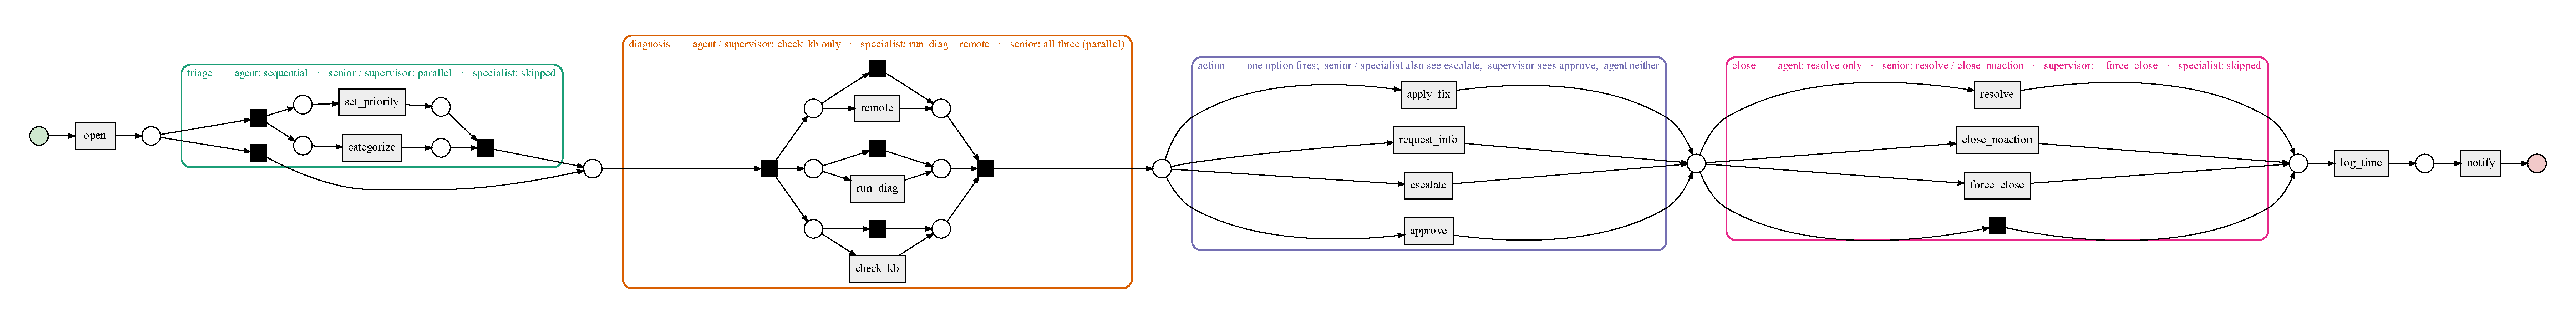
\includegraphics[width=\linewidth]{servicedesk_dejure}
    \caption{The designed (de-jure) workflow --- the union of what all four roles can do --- annotated with how each role restricts the triage, diagnosis, action, and close blocks.}
  \end{subfigure}\\[3pt]
  \begin{subfigure}{\linewidth}
    \centering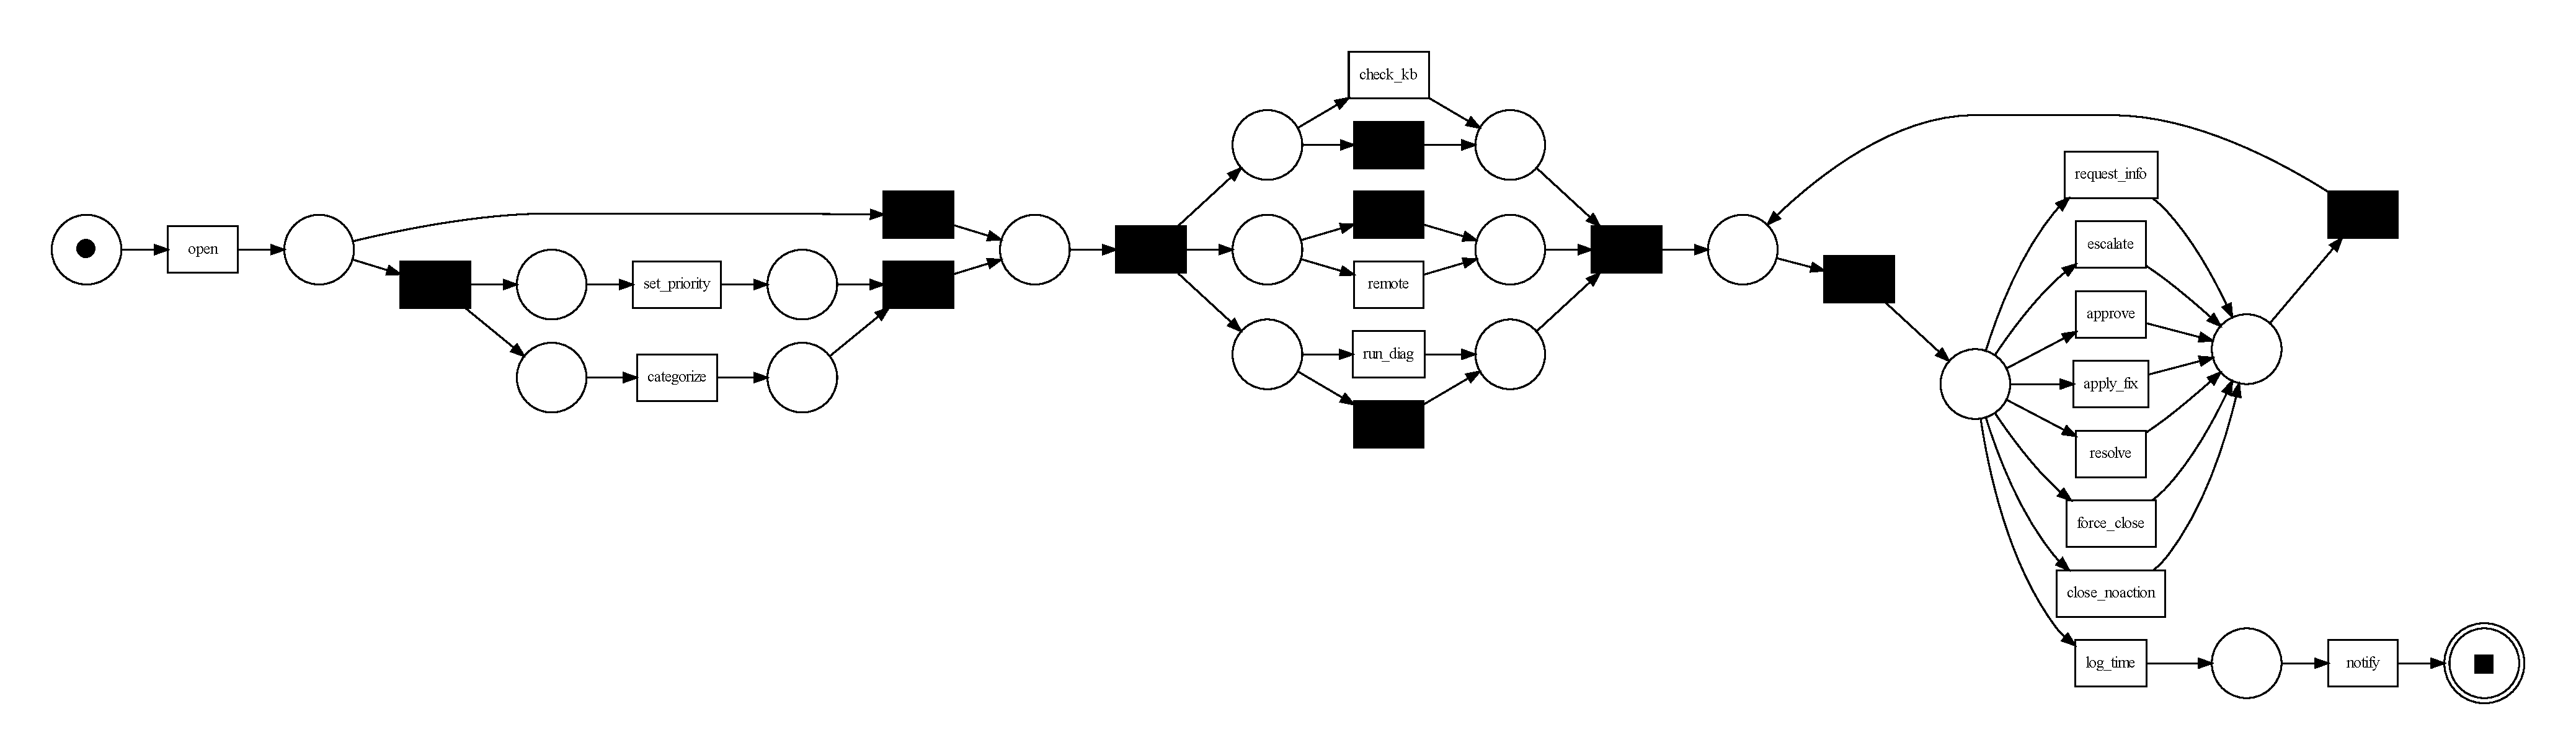
\includegraphics[width=0.9\linewidth]{servicedesk_global}
    \caption{One model mined from the whole log (roles conflated).}
  \end{subfigure}\\[3pt]
  \begin{subfigure}{0.49\linewidth}
    \centering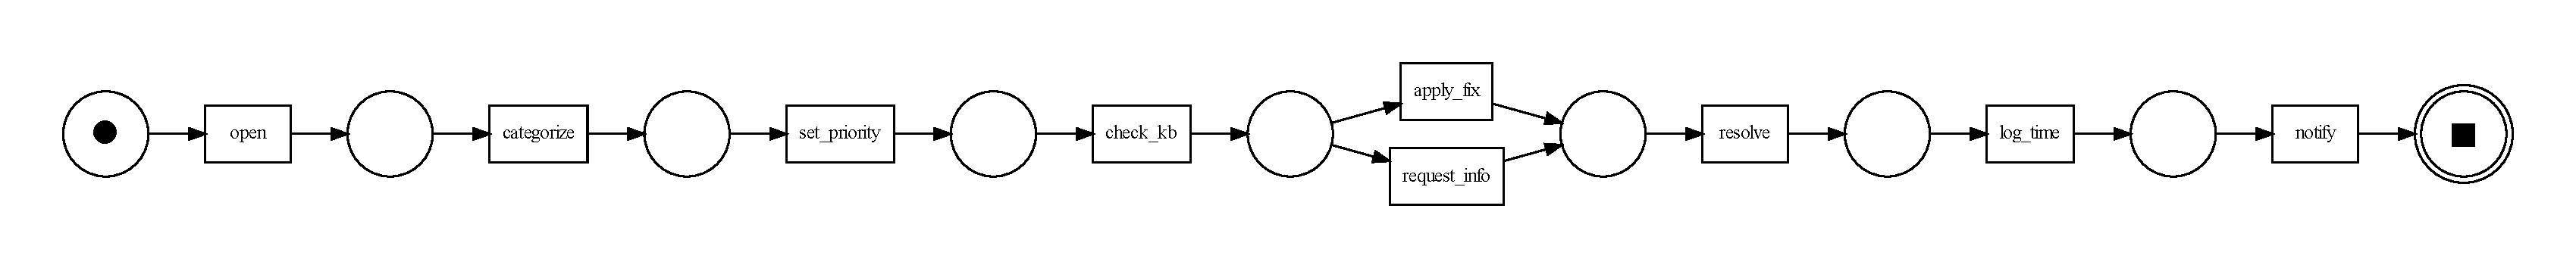
\includegraphics[width=\linewidth]{servicedesk_kappa_agent}
    \caption{$\kappa$ view --- agent.}
  \end{subfigure}\hfill
  \begin{subfigure}{0.49\linewidth}
    \centering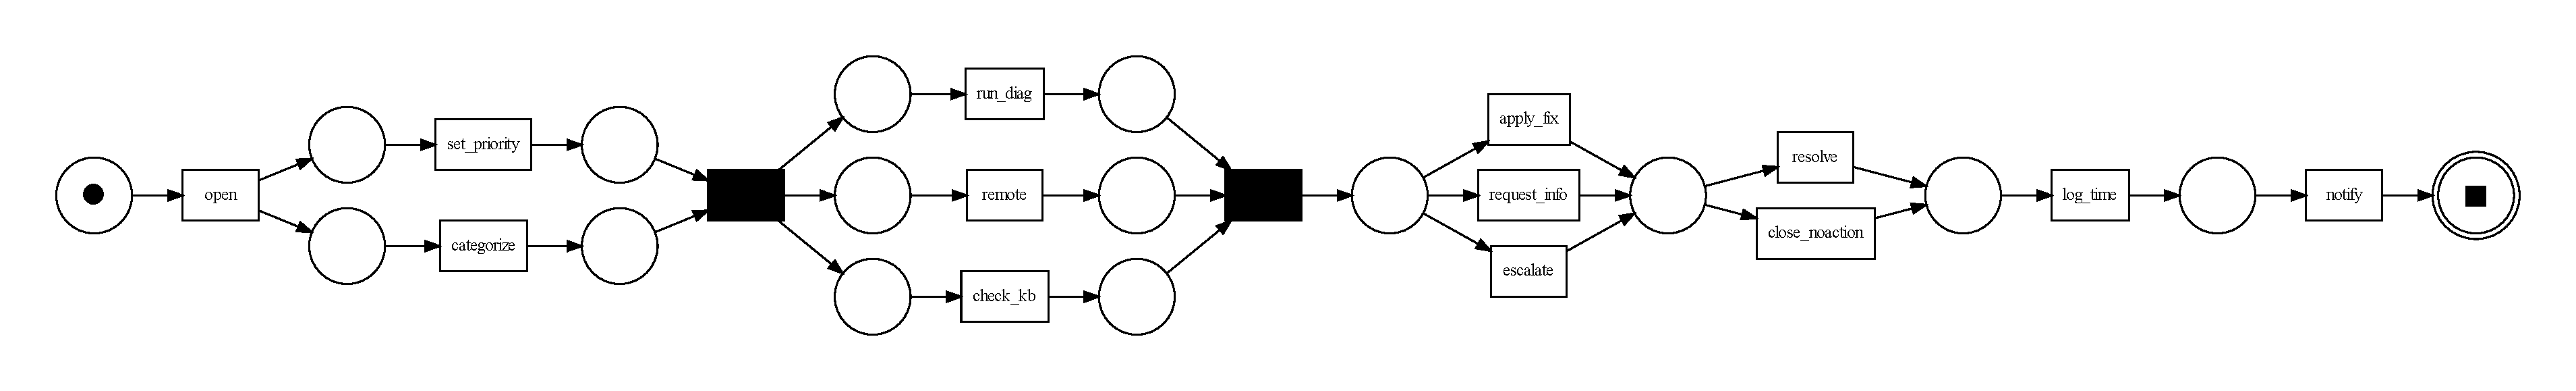
\includegraphics[width=\linewidth]{servicedesk_kappa_senior}
    \caption{$\kappa$ view --- senior.}
  \end{subfigure}\\[3pt]
  \begin{subfigure}{0.49\linewidth}
    \centering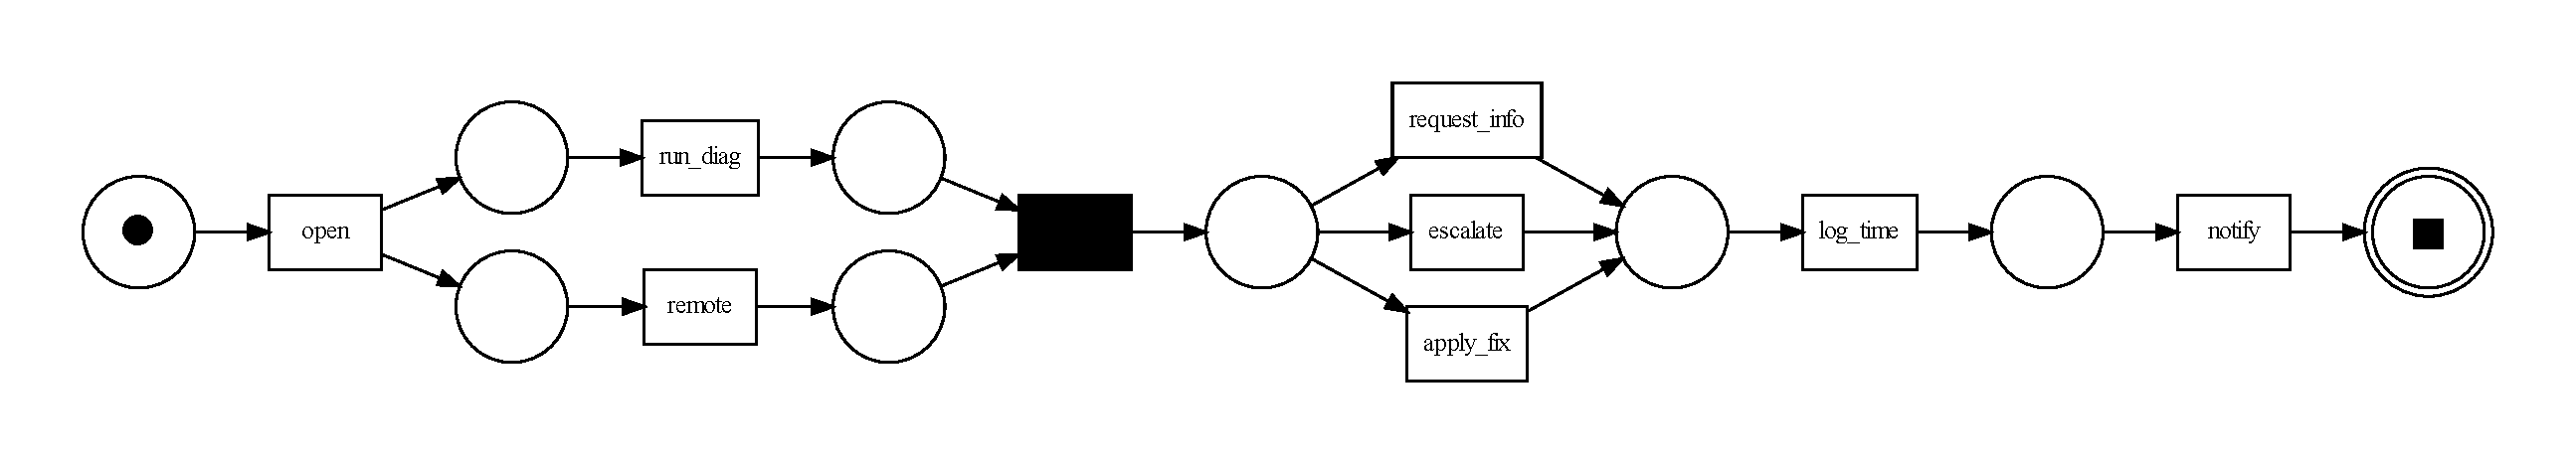
\includegraphics[width=\linewidth]{servicedesk_kappa_specialist}
    \caption{$\kappa$ view --- specialist.}
  \end{subfigure}\hfill
  \begin{subfigure}{0.49\linewidth}
    \centering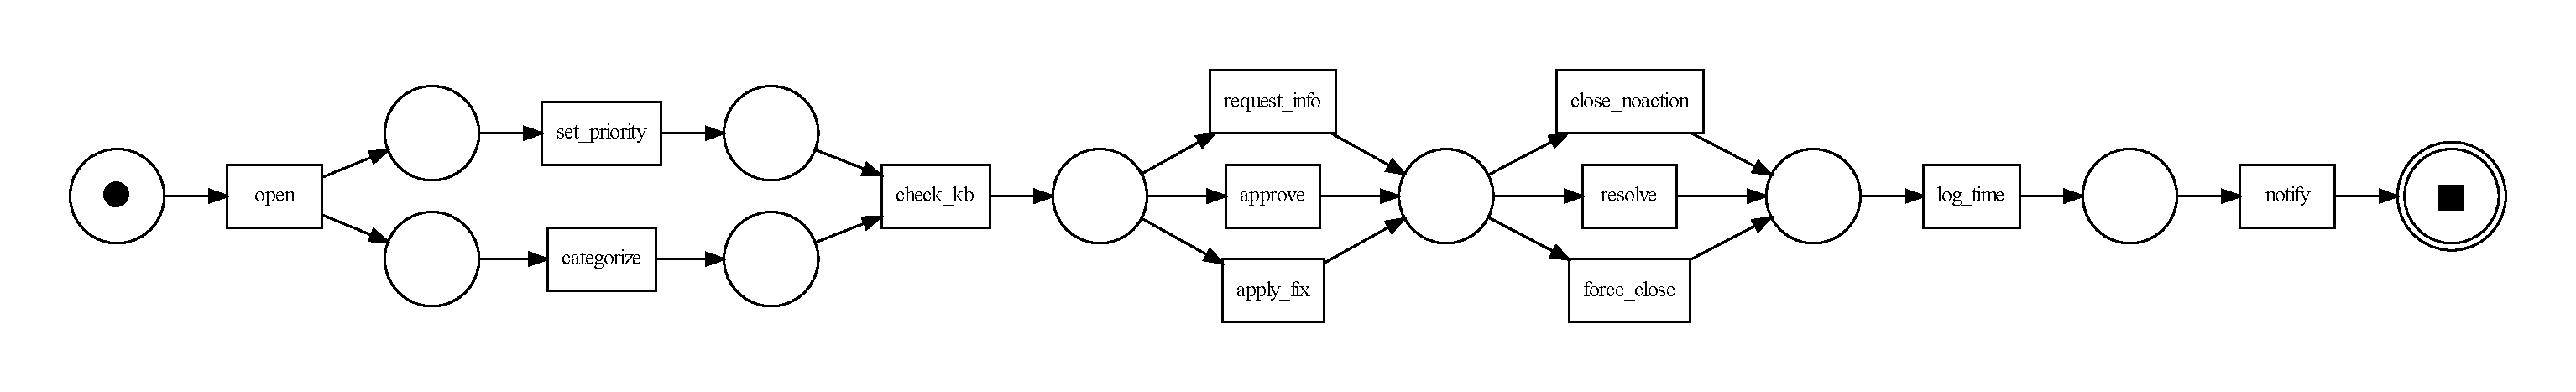
\includegraphics[width=\linewidth]{servicedesk_kappa_supervisor}
    \caption{$\kappa$ view --- supervisor.}
  \end{subfigure}
  \caption{Service-desk workflow at $p=0$: (a) the designed (de-jure) model, the union of all four roles; (b) one model mined over the whole log; (c--f) the four models $\kappa$ induces, one per hidden role.
  Places are circles, transitions are boxes, silent transitions are filled.}
  \label{fig:scenario-models}
\end{figure}

Figure~\ref{fig:scenario-models}(a) is the de-jure model: the four roles share one skeleton and differ only in how each block is constrained --- an agent runs triage in sequence and can only \texttt{resolve}, a senior and a supervisor run triage in parallel, a specialist drops triage and close, and only a supervisor sees \texttt{approve} and \texttt{force\_close}.
The rest of Figure~\ref{fig:scenario-models} contrasts one global model with the four models $\kappa$ induces at $p=0$.
The global model is visibly loose --- it makes triage optional, turns diagnosis into a three-way parallel block with skips, and merges the action and close steps into one seven-way choice with a loop back --- whereas each of $\kappa$'s models matches one role exactly: the agent model is a plain sequence, the senior model runs triage and a wide diagnosis block in parallel and offers \texttt{escalate}, the specialist model has neither a triage nor a close step, and only the supervisor model has \texttt{approve} and \texttt{force\_close}.

\begin{table}[t]
  \centering
  \caption{Service-desk case study: ARI and translucent F1 for every approach at each enabled-set noise level $p$ (mean over three seeds); the best value in each column is in \textbf{bold}.}
  \label{tab:case}
  \scriptsize\setlength{\tabcolsep}{3pt}
  \resizebox{\linewidth}{!}{\begin{tabular}{lrrrrrrrrrr}
\toprule
 & ARI $p{=}0$ & tr.\ F1 $p{=}0$ & ARI $p{=}0.05$ & tr.\ F1 $p{=}0.05$ & ARI $p{=}0.1$ & tr.\ F1 $p{=}0.1$ & ARI $p{=}0.15$ & tr.\ F1 $p{=}0.15$ & ARI $p{=}0.2$ & tr.\ F1 $p{=}0.2$ \\
\midrule
global & 0.000 & 0.566 & 0.000 & 0.741 & 0.000 & 0.668 & 0.000 & 0.699 & 0.000 & 0.645 \\
$\kappa$ (ours) & \textbf{1.000} & \textbf{1.000} & 0.563 & 0.944 & 0.299 & 0.952 & 0.127 & 0.944 & 0.063 & \textbf{0.936} \\
$\kappa$ + support (ours) & \textbf{1.000} & \textbf{1.000} & \textbf{0.996} & \textbf{0.979} & \textbf{0.988} & \textbf{0.961} & \textbf{0.973} & 0.902 & \textbf{0.951} & 0.914 \\
CF-TC Ward (GT) & 0.640 & 0.985 & 0.719 & 0.953 & 0.732 & 0.943 & 0.728 & \textbf{0.947} & 0.722 & 0.902 \\
CTX-TC (GT) & 0.630 & 0.985 & 0.813 & 0.974 & 0.886 & 0.956 & 0.765 & 0.936 & 0.714 & 0.917 \\
EN-TC (GT) & 0.753 & 0.990 & 0.711 & 0.896 & 0.806 & 0.933 & 0.577 & 0.891 & 0.573 & 0.849 \\
D2V-TC (GT) & 0.720 & 0.948 & 0.401 & 0.846 & 0.564 & 0.786 & 0.551 & 0.832 & 0.670 & 0.844 \\
ATTR-TC clean (GT) & 0.806 & 0.952 & 0.655 & 0.756 & 0.649 & 0.769 & 0.906 & 0.841 & 0.891 & 0.806 \\
ATTR-TC noisy (GT) & 0.117 & 0.646 & 0.049 & 0.658 & 0.024 & 0.713 & 0.017 & 0.662 & 0.006 & 0.721 \\
variant discovery & 0.224 & 0.949 & 0.222 & 0.946 & 0.222 & 0.894 & 0.224 & 0.927 & 0.224 & 0.908 \\
translucent-variant grouping & 0.272 & 0.949 & 0.133 & 0.945 & 0.066 & 0.942 & 0.026 & 0.937 & 0.014 & 0.933 \\
ATTR-TC oracle (GT)$^{\dagger}$ & 1.000 & 1.000 & 1.000 & 0.983 & 1.000 & 0.973 & 1.000 & 0.949 & 1.000 & 0.937 \\
\bottomrule
\end{tabular}
}
\end{table}

Table~\ref{tab:case} shows the effect of noise.
At $p=0$, $\kappa$ recovers all four roles exactly (ARI $1.00$, four views); as $p$ rises its ARI falls to $0.31$ and $0.08$ and its view count grows from $4$ to $412$ and $659$, because each corrupted trace becomes its own view.
The control-flow baselines behave oppositely: their partition is read from the executed activities, which noise never touches, so their ARI stays around $0.6$--$0.85$ across all noise levels --- and never recovers the roles, which differ mainly in availability, not execution.
Attribute clustering on the clean attributes stays at ARI $1.00$ throughout, since \texttt{role} is unaffected by enabled-set noise --- again, only because it was recorded and $k$ was supplied.
$\kappa$'s translucent F1 nevertheless stays high ($1.00$ then ${\approx}0.94$) as its ARI collapses: each noise fragment is tiny and still modelled faithfully; what degrades is the grouping, not the per-group models.

\paragraph{Limitations.}
The synthetic logs give $\kappa$ a clean hidden context and thus its best case; real contexts overlap and drift.
$\kappa$ depends entirely on the fidelity of the enabled sets, as the case study shows, and reaches parity with attribute slicing once the context is recorded and $k$ is known.
It has no loop operator and over-segments unbounded rework (the \emph{rework loop} log: four views for zero hidden contexts), all models use a single miner (IMtf), and a few very loose sub-models fall back to token-based replay and earn no translucent-quality credit.
Overall, $\kappa$ recovers hidden availability context exactly and parameter-free when the enabled sets are trustworthy, and its per-view models are the most faithful to the enabled behaviour; its reliance on that single signal is also its main weakness.

\appendix
\section{Additional detail}
\label{sec:appendix}
Figure~\ref{fig:scenario} resolves the case study by metric --- $\kappa$'s adjusted Rand index collapses as noise rises while its translucent fitness and F1 stay high, and the control-flow baselines are flat throughout.
Table~\ref{tab:quality-cw} is the case-weighted variant of Table~\ref{tab:quality}: weighting the nine logs by their case counts does not change the ordering.

\begin{figure}[htbp]
  \centering
  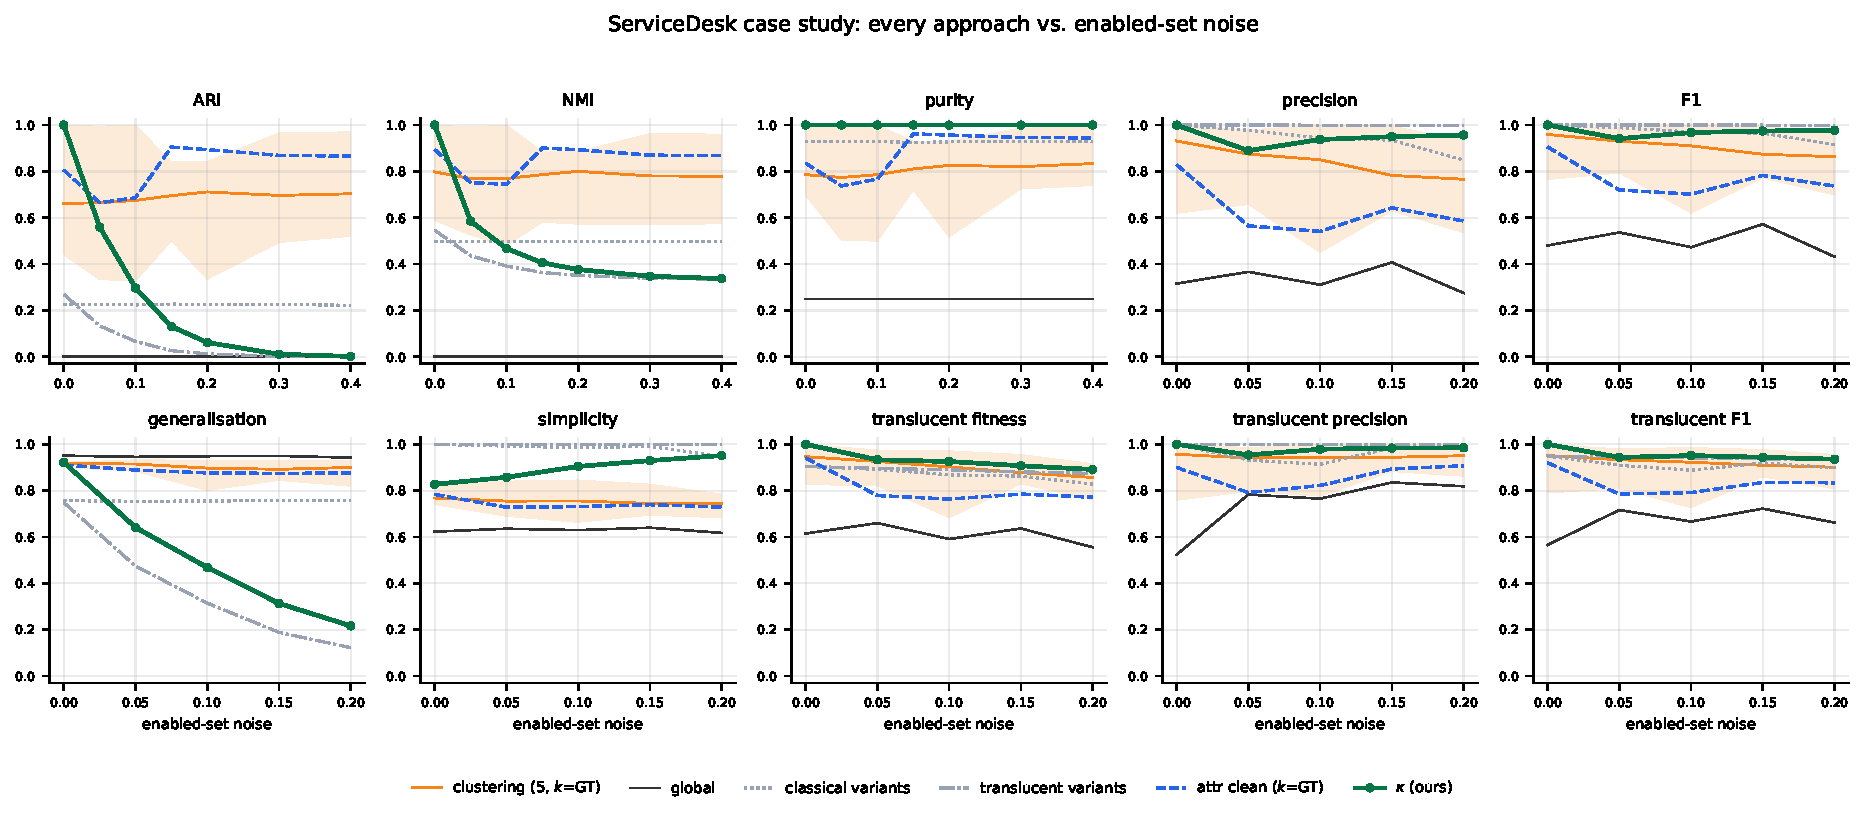
\includegraphics[width=\linewidth]{fig_scenario}
  \caption{Service-desk case study: each metric against the enabled-set noise level $p$.
  $\kappa$ (bold); the five $k=\mathrm{GT}$ clustering baselines as a min--max band with their mean; \emph{ATTR-TC clean} ($k=\mathrm{GT}$), \emph{variant discovery}, and \emph{global} as named lines.}
  \label{fig:scenario}
\end{figure}

\begin{table}[htbp]
  \centering
  \caption{Case-weighted variant of Table~\ref{tab:quality}: each log weighted by its case count.}
  \label{tab:quality-cw}
  \footnotesize\setlength{\tabcolsep}{4pt}
  \resizebox{\linewidth}{!}{\begin{tabular}{lrrrrrrrr}
\toprule
 & \#mdl & prec. & F1 & gen. & simp. & tr.\ fit. & tr.\ prec. & tr.\ F1 \\
\midrule
global & 1.000 & 0.944 & 0.969 & \textbf{0.966} & 0.679 & 0.888 & 0.983 & 0.932 \\
$\kappa$ (ours) & 4.108 & 0.967 & 0.982 & 0.940 & 0.786 & \textbf{0.987} & \textbf{0.999} & \textbf{0.992} \\
$\kappa$ + support (ours) & 4.108 & 0.967 & 0.982 & 0.940 & 0.786 & \textbf{0.987} & \textbf{0.999} & \textbf{0.992} \\
CF-TC $k$-means (GT) & 4.108 & 0.951 & 0.974 & 0.940 & 0.760 & 0.913 & 0.998 & 0.953 \\
CF-TC Ward (GT) & 4.108 & 0.917 & 0.956 & 0.939 & 0.757 & 0.932 & 0.994 & 0.962 \\
CTX-TC (GT) & 4.108 & 0.881 & 0.920 & 0.936 & 0.761 & 0.895 & 0.951 & 0.922 \\
EN-TC (GT) & 4.108 & 0.863 & 0.911 & 0.942 & 0.773 & 0.910 & 0.923 & 0.915 \\
D2V-TC (GT) & 4.108 & 0.805 & 0.884 & 0.934 & 0.723 & 0.884 & 0.908 & 0.895 \\
ATTR-TC clean (GT) & 4.113 & 0.946 & 0.971 & 0.942 & 0.738 & 0.953 & 0.990 & 0.971 \\
ATTR-TC noisy (GT) & 4.113 & 0.843 & 0.913 & 0.932 & 0.683 & 0.901 & 0.971 & 0.934 \\
ATTR-TC all (GT) & 4.113 & 0.883 & 0.937 & 0.928 & 0.711 & 0.932 & 0.974 & 0.952 \\
variant discovery & 590.963 & \textbf{0.993} & \textbf{0.996} & 0.678 & \textbf{0.998} & 0.852 & \textbf{0.999} & 0.919 \\
translucent-variant grouping & 661.264 & \textbf{0.993} & \textbf{0.996} & 0.642 & \textbf{0.998} & 0.852 & \textbf{0.999} & 0.919 \\
ATTR-TC oracle (GT)$^{\dagger}$ & 4.113 & 0.972 & 0.985 & 0.940 & 0.779 & 0.993 & 1.000 & 0.996 \\
\bottomrule
\end{tabular}
}
\end{table}

\clearpage
\footnotesize
\begin{multicols}{2}
\setlength{\itemsep}{1pt}
\begin{thebibliography}{99}
\bibitem{song2008} M.\ Song, C.~W.\ G{\"u}nther, W.~M.~P.\ van der Aalst.
  Trace clustering in process mining. In \emph{BPM Workshops}, LNBIP 17,
  109--120. Springer, 2008.
\bibitem{bose2009} R.~P.~J.~C.\ Bose, W.~M.~P.\ van der Aalst. Context aware
  trace clustering: towards improving process mining results. In \emph{SDM},
  401--412. SIAM, 2009.
\bibitem{dekoninck2018} P.\ De~Koninck, S.\ vanden~Broucke, J.\ De~Weerdt.
  act2vec, trace2vec, log2vec, and model2vec: representation learning for
  business processes. In \emph{BPM}, LNCS 11080, 305--321. Springer, 2018.
\bibitem{greco2006} G.\ Greco, A.\ Guzzo, L.\ Pontieri, D.\ Sacc{\`a}.
  Discovering expressive process models by clustering log traces.
  \emph{IEEE TKDE} 18(8):1010--1027, 2006.
\bibitem{garciabanuelos2014} L.\ Garc{\'i}a-Ba{\~n}uelos, M.\ Dumas,
  M.\ La~Rosa, J.\ De~Weerdt, C.~C.\ Ekanayake. Controlled automated discovery
  of collections of business process models. \emph{Information Systems}
  46:85--101, 2014.
\bibitem{carmona2018} J.\ Carmona, B.~F.\ van Dongen, A.\ Solti, M.\ Weidlich.
  \emph{Conformance Checking -- Relating Processes and Models}. Springer, 2018.
\bibitem{vanderaalst2016} W.~M.~P.\ van der Aalst. \emph{Process Mining -- Data
  Science in Action}. 2nd ed., Springer, 2016.
\bibitem{adriansyah2014} A.\ Adriansyah. \emph{Aligning Observed and Modeled
  Behavior}. PhD thesis, Eindhoven University of Technology, 2014.
\bibitem{beyel2024tp} H.~H.\ Beyel, W.~M.~P.\ van der Aalst. Translucent
  precision: exploiting enabling information to evaluate the quality of process
  models. In \emph{RCIS}, LNBIP 513, 29--37. Springer, 2024.
\bibitem{beyel2025ta} H.~H.\ Beyel, C.~T.\ Schwanen, W.~M.~P.\ van der Aalst.
  Translucent alignments. In \emph{CAiSE}, 167--184. Springer, 2025.
\bibitem{beyel2024tar} H.~H.\ Beyel, W.~M.~P.\ van der Aalst. Improving process
  discovery using translucent activity relationships. In \emph{BPM}, LNCS 14940,
  146--163. Springer, 2024.
\bibitem{beyel2024ag} H.~H.\ Beyel, M.\ Beyel, W.~M.~P.\ van der Aalst.
  ActivityGen: extracting enabled activities from screenshots. In \emph{ECAI},
  2024.
\bibitem{rousseeuw1987} P.~J.\ Rousseeuw. Silhouettes: a graphical aid to the
  interpretation and validation of cluster analysis. \emph{J.\ Comput.\ Appl.\
  Math.} 20:53--65, 1987.
\bibitem{lemikolov2014} Q.\ Le, T.\ Mikolov. Distributed representations of
  sentences and documents. In \emph{ICML}, 1188--1196. PMLR, 2014.
\end{thebibliography}
\end{multicols}

\end{document}
